\chapter{Création du typon}
Pendant la création de ce typon, on est amenés à modifier la schématique sous Orcad pour ajouter:
\begin{itemize}
    \item le pont diviseur en entrée;
    \item le strap et la résistance pour mesurer l’impédance d’entrée;
    \item les connecteurs pour les alimentations, l’entrée et la sortie;
    \item les capacités de découplage entre les étages;
\end{itemize}

Il nous faut aussi créer un schéma sur une seule page:

\begin{center}
    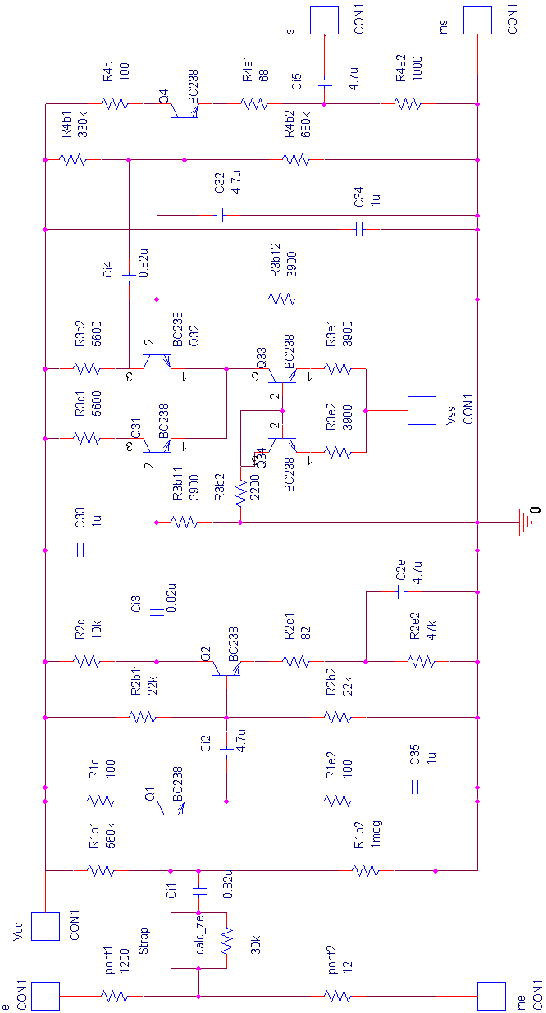
\includegraphics[height=24cm]{images/circuit-pour-typon}

    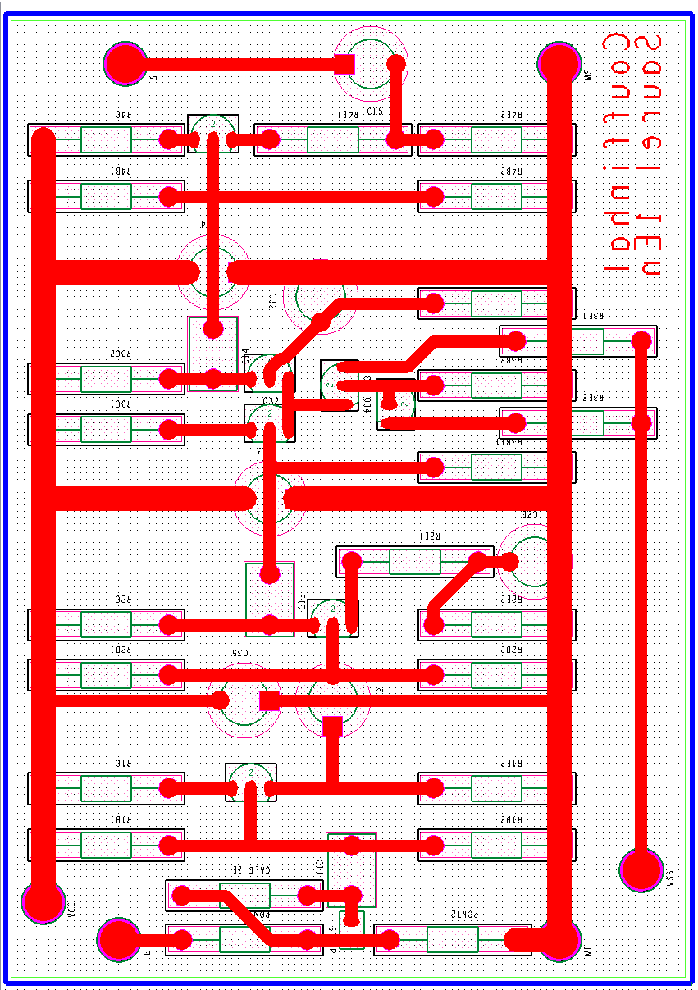
\includegraphics[height=24cm]{images/typon}
\end{center}
